\chapter{Desarrollo}\label{ch:Desarrollo}
\section{Estructura del Simulador}
En el desarrollo del prototipo de simulador de laboratorio de Química Inorgánica en Realidad Virtual, la organización del proyecto en Unity desempeña un papel crucial para mantener un entorno de desarrollo estructurado, escalable y mantenible. Al crear un proyecto nuevo en Unity, se genera una carpeta principal llamada Assets, que contiene todos los recursos necesarios para el correcto funcionamiento del simulador.

\begin{figure}[thbp]
    \centering
    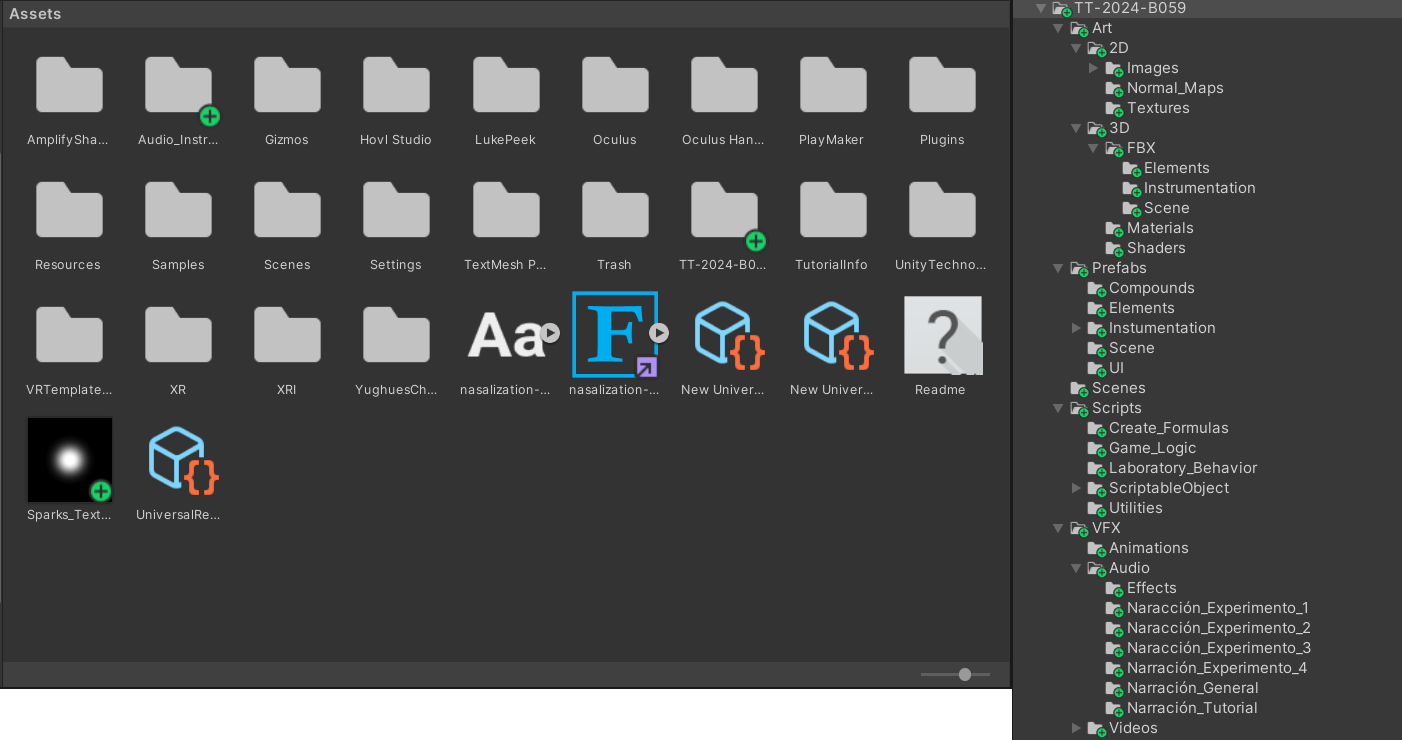
\includegraphics[width=0.8\textwidth, height = 7cm]{img/chapter04/Estructura.png}
    \caption{Assets del Simulador}
    \label{fig:Assets_del_Simulador}
\end{figure}

Esta carpeta se subdivide en varias carpetas específicas según su propósito, como se detalla a continuación:

\begin{enumerate} [I. ]
    \item \textit{\textbf{Art}}:
    
    Esta carpeta contiene los recursos gráficos utilizados en el simulador, divididos en dos subcarpetas principales:
    \begin{itemize}
        \item \textbf{2D}: Incluye imágenes, mapas normales y texturas utilizadas para enriquecer los elementos visuales del entorno.
        \newpage
        \item \textbf{3D}: Contiene modelos tridimensionales organizados en:
        \begin{itemize}
            \item FBX: Modelos de elementos, instrumental y escenas del laboratorio.
            \item Materials: Materiales aplicados a los modelos para simular texturas y propiedades físicas.
            \item Shaders\_Graphs: Gráficos de sombreado personalizados que mejoran el realismo del entorno virtual.
        \end{itemize}
    \end{itemize}

    \item \textit{\textbf{Prefabs}}:
    
    Los prefabs son objetos prediseñados con configuraciones preestablecidas, lo que permite reutilizarlos en múltiples escenas. Están organizados en:
    \begin{itemize}
        \item \textbf{Compounds}: Compuestos químicos modelados y configurados con comportamientos específicos.
        \item \textbf{Elements}: Elementos químicos individuales listos para ser utilizados en las simulaciones.
        \item \textbf{Instrumentation}: Herramientas e instrumentos del laboratorio como matraces, tubos de ensayo y mecheros.
        \item \textbf{Scene}: Componentes específicos para gestionar aspectos visuales y funcionales de las escenas.
        \item \textbf{UI}: Elementos de interfaz de usuario diseñados para facilitar la interacción.
    \end{itemize}

    \item \textit{\textbf{Scenes:}}
    
    Esta carpeta contiene todas las escenas creadas para el simulador
    \begin{itemize}
        \item \textbf{Experimentos}: Cada experimento tiene su propia escena, diseñada específicamente para simular procedimientos y reacciones químicas.
        \item \textbf{Tutorial}: Provee instrucciones guiadas para familiarizar al usuario con el simulador y las actividades.
        \item \textbf{Hub}: Actúa como un menú principal donde el usuario puede navegar hacia diferentes experimentos o tutoriales.
    \end{itemize}

    \item \textit{\textbf{Scripts}}:
    
    Contiene todos los scripts de código fuente en lenguaje C\#, organizados según su funcionalidad en las siguientes subcarpetas:
    \begin{itemize}
        \item \textbf{Create\_Formulas}: Scripts para crear y gestionar las fórmulas químicas utilizadas en el simulador.
        \item \textbf{Game\_Logic}: Lógica general del simulador, como eventos y reglas específicas.
        \item \textbf{Laboratory\_Behavior}: Comportamientos de los elementos interactivos del laboratorio.
        \item \textbf{ScriptableObject}: Configuraciones y datos reutilizables en formato ScriptableObject.
        \item \textbf{Utilities}: Scripts auxiliares que apoyan funcionalidades generales del simulador.
    \end{itemize}
    Los scripts se desarrollan siguiendo principios de programación orientada a objetos, aplicando el uso de máquinas de estado para la gestión de escenas y experimentos.

    \item \textit{\textbf{VFX}}:
    
    Esta carpeta contiene los efectos visuales y auditivos que mejoran la experiencia inmersiva del usuario:
    \begin{itemize}
        \item \textbf{Animations}: Animaciones aplicadas a modelos y elementos interactivos.
        \item \textbf{Audio}: Archivos de sonido organizados en:
        \begin{itemize}
            \item Effects: Efectos de sonido específicos.
            \item Narraciones: Audio dividido en narraciones para tutoriales y experimentos.
        \end{itemize}
        \item \textbf{Videos}: Clips de video utilizados para complementar la experiencia educativa.
    \end{itemize}    
\end{enumerate}

\section{Ambiente Virtual} \label{sec:Ambiente_Virtual}

El ambiente virtual desarrollado para el simulador proporciona un espacio interactivo e inmersivo donde los usuarios pueden realizar diversos experimentos de química inorgánica. Este entorno simula un laboratorio moderno e incluye los elementos necesarios para recrear prácticas científicas de manera eficiente y educativa.
\subsection{Diseño del entorno 3D}
El laboratorio consta de los siguientes elementos principales:
\begin{itemize}
    \item \textbf{Mesa de trabajo}: Área central donde se llevan a cabo los experimentos. Diseñada para proporcionar un espacio virtual amplio y funcional que facilita la manipulación de los objetos.
    \item \textbf{Modelos atómicos de los elementos}: Representaciones tridimensionales de los átomos, diseñadas para ilustrar sus estructuras y propiedades.
    \begin{figure}[thbp]
        \centering
        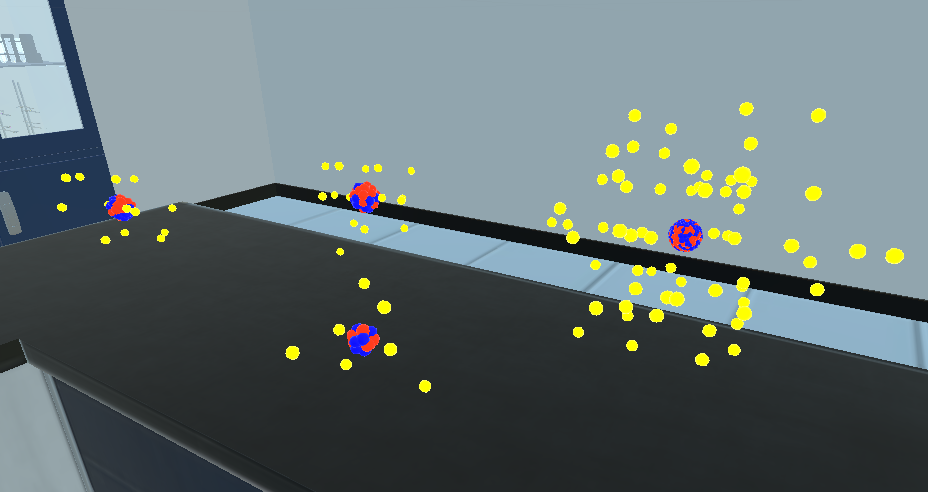
\includegraphics[width=0.6\textwidth, height = 6cm]{img/chapter04/Elementos.png}
        \caption{Modelos de Elementos Químicos}
        \label{fig:Elementos_Químicos}
    \end{figure}
    \newpage
    \item \textbf{Tabla periódica interactiva}: Permite al usuario explorar los elementos químicos de forma dinámica. Al seleccionar un elemento, se despliega información relevante y un modelo atómico tridimensional.
    \begin{figure}[thbp]
        \centering
        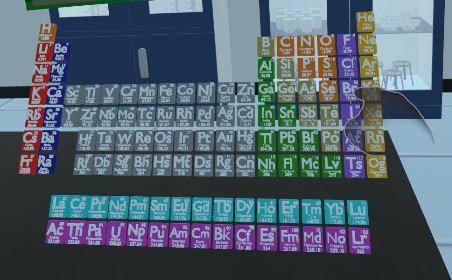
\includegraphics[width=0.6\textwidth, height = 5cm]{img/chapter05/Tabla_Periodica.png}
        \caption{Tabla Periódica}
        \label{fig:Tabla_Periódica}
    \end{figure}

    \item \textbf{Instrumental necesario}: Incluye matraces, tubos de ensayo, mecheros y demás herramientas esenciales, modeladas en detalle para reflejar con precisión el equipo utilizado en laboratorios reales.
    \begin{figure}[thbp]
        \centering
        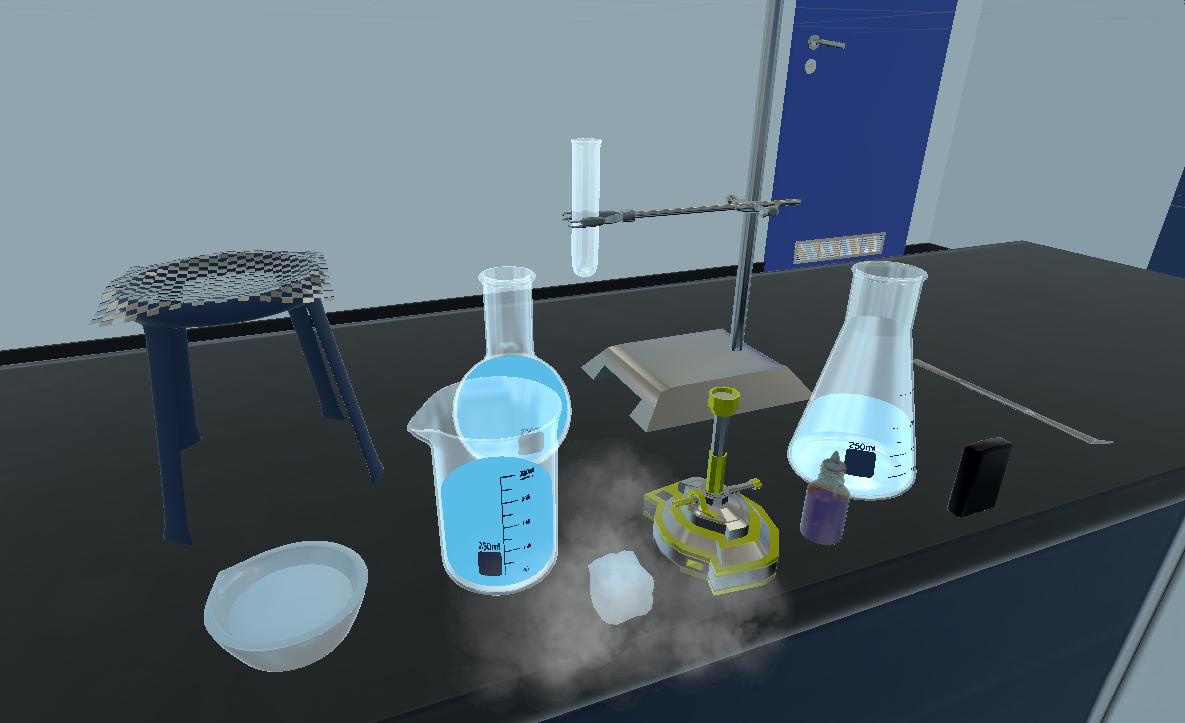
\includegraphics[width=0.6\textwidth, height = 6cm]{img/chapter04/Instrumental.png}
        \caption{Instrumental de Laboratorio}
        \label{fig:Instrumental_De_Laboratorio}
    \end{figure}
    \newpage
    \item \textbf{Modelos de compuestos químicos}: Reproducciones de los compuestos que se generan durante los experimentos, mostrando sus características visuales de manera precisa.
    \begin{figure}[thbp]
        \centering
        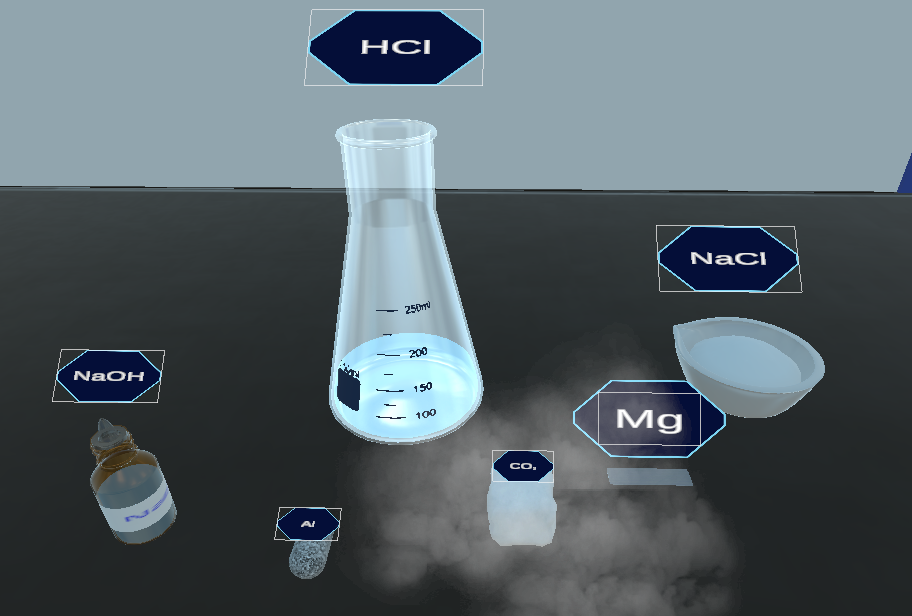
\includegraphics[width=0.6\textwidth, height = 6cm]{img/chapter04/Compuestos.png}
        \caption{Compuestos Químicos}
        \label{fig:Compuestos_Químicos}
    \end{figure}
\end{itemize}

Todo el modelado 3D fue desarrollado utilizando Blender, una herramienta ampliamente reconocida en la industria por su capacidad para crear modelos tridimensionales detallados y eficientes. Las texturas y materiales de estos modelos se trabajaron en GIMP.

\subsection{Efectos Visuales (VFX)}
Para mejorar la inmersión y reforzar la representación de las reacciones químicas y los fenómenos experimentales, se diseñaron una variedad de efectos de partículas. Entre los principales se encuentran:
\begin{itemize}
    \item \textbf{Humo y Vapores}: Representan las liberaciones de gases en ciertas reacciones químicas.
    \item \textbf{Fuego y Chispas}: Simulan encendidos de mecheros y otras reacciones exotérmicas.
    \item \textbf{Niebla}: Utilizada como un efecto visual en reacciones específicas.
\end{itemize}
\begin{figure}[thbp]
    \centering
    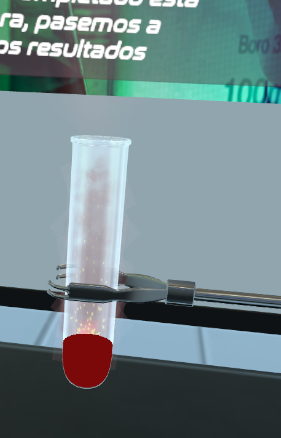
\includegraphics[width=0.6\textwidth, height = 6cm]{img/chapter04/VFX.png}
    \caption{Efectos de Partículas}
    \label{fig:Diversos_Efectos_Visuales}
\end{figure}
Estos efectos se crearon utilizando el Unity Particle System y shaders personalizados para lograr una integración fluida con el entorno.

\subsection{Efectos de Sonido}
El sonido juega un papel fundamental en la inmersión sensorial del simulador. Se incorporaron diversos efectos sonoros para acompañar las interacciones y eventos del laboratorio, incluyendo:
\begin{itemize}
    \item \textbf{Cristales}: Simulan el sonido de recipientes de vidrio al ser manipulados o chocados.
    \item \textbf{Burbujeos y flujo de agua}: Representan procesos químicos y líquidos en movimiento.
    \item \textbf{Fuego y gas}: Emulan encendidos de mecheros y escapes controlados de gases.
\end{itemize}

Los sonidos fueron seleccionados y editados para sincronizarse con precisión en tiempo real mediante el sistema de eventos de Unity. Esto asegura que cada acción del usuario esté acompañada de una respuesta auditiva coherente y realista.
\subsection{Instrucciones guiadas con voz}
Para las instrucciones paso a paso, se utilizó el servicio en línea SpeechGen.io, el cual permitió generar voces claras y dinámicas en varios idiomas. Este sistema se integró para:
\begin{itemize}
    \item Proporcionar guías auditivas que refuercen las instrucciones visuales.
    \item Sincronizar las instrucciones de voz con las acciones y eventos dentro del laboratorio, mejorando la accesibilidad y la experiencia del usuario.
\end{itemize}

\section{Diseño de Interfaz de Usuario}
El diseño de la interfaz de usuario (IU) para el simulador se desarrolló con un enfoque en maximizar la funcionalidad y la accesibilidad dentro del entorno de realidad virtual (RV), adaptándose a las necesidades de un laboratorio químico interactivo. Estas interfaces, aunque densas en información, fueron optimizadas para que los usuarios puedan acceder fácilmente a datos relevantes y operar de manera eficiente en un entorno inmersivo.

\subsection{Hub de selección}
Sirve como el punto de entrada al simulador, diseñado para ofrecer una navegación jerarquía y estructurada:
\begin{itemize}
    \item \textbf{Pantalla inicial}: Contiene dos botones principales: Tutorial y Experimentos.
    \item \textbf{Pantalla de selección de experimentos}: Presenta 4 botones, cada uno correspondiente a un experimento disponible y un quinto botón para regresar al menú principal.
    \item \textbf{Pantalla Tutorial-Experimentos}: Proporciona una descripción general de la selección, con su imagen de referencia y dos opciones de navegación, regresar y confirmar.
\end{itemize}
\begin{figure}[thbp]
    \centering
    \begin{subfigure}[b]{0.4\linewidth}
        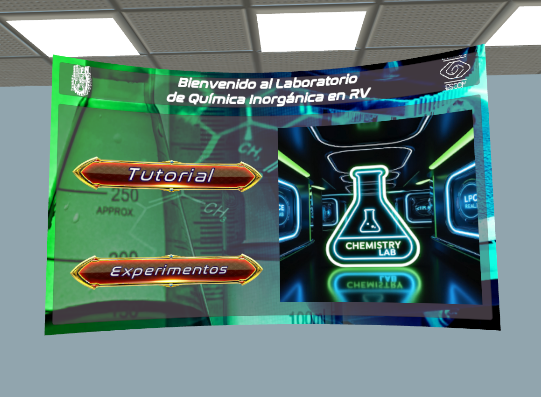
\includegraphics[width=\linewidth, height = 5cm]{img/chapter04/UI_Hub.png}
        \caption{Pantalla Principal Hub}
        \label{fig:Hub_Principal}
    \end{subfigure}
    \begin{subfigure}[b]{0.4\linewidth}
        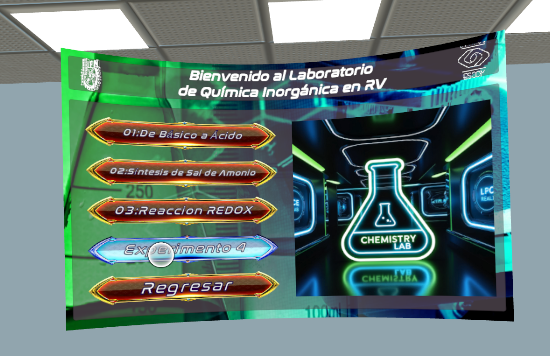
\includegraphics[width=\linewidth, height = 5cm]{img/chapter04/UI_Hub_Experiments.png}
        \caption{Pantalla Selección Experimento}
        \label{fig:Hub_Experimentos}
    \end{subfigure}
    \begin{subfigure}[b]{0.4\linewidth}
        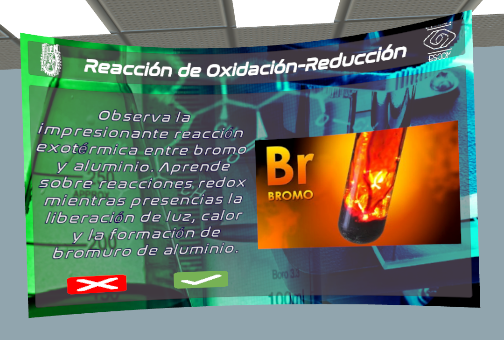
\includegraphics[width=\linewidth, height = 5cm]{img/chapter04/UI_Hub_Experiment.png}
        \caption{Pantalla Información Experimento}
        \label{fig:Hub_Experimento}
    \end{subfigure}
    \caption{IU Hub}
\end{figure}
\newpage
\subsection{Información principal}
Centraliza la información operativa de cada experimento, proporcionando:
\begin{itemize}
    \item Instrucciones detalladas
    \item Soporte visual
    \item Ecuaciones químicas
\end{itemize}
\begin{figure}[thbp]
    \centering
    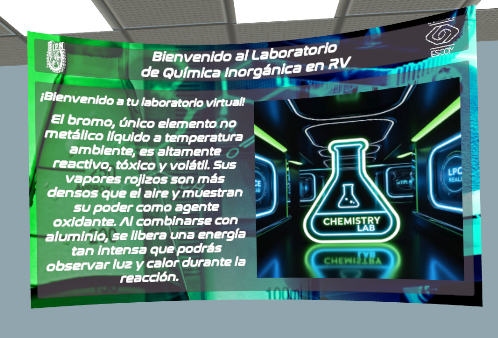
\includegraphics[width=0.6\textwidth, height = 6cm]{img/chapter04/UI_Principal.png}
    \caption{IU Principal}
    \label{fig:Principal_IU}
\end{figure}

\subsection{Elementos}
Se focaliza en proporcionar datos contextuales sobre el último elemento químico seleccionado
\begin{figure}[thbp]
    \centering
    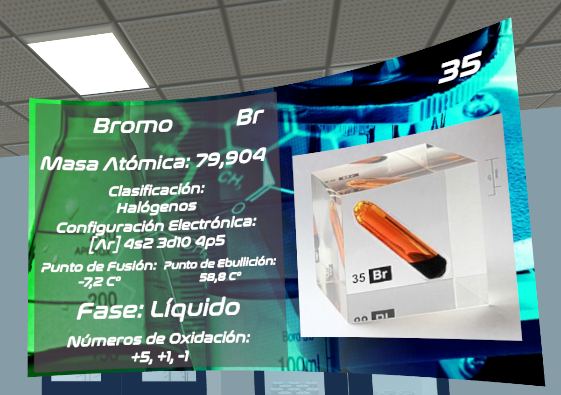
\includegraphics[width=0.6\textwidth, height = 6cm]{img/chapter04/UI_Elements.png}
    \caption{IU Elementos}
    \label{fig:Elementos_IU}
\end{figure}

\subsection{Compuestos}
Presenta información sobre el último compuesto generado.
\begin{figure}[thbp]
    \centering
    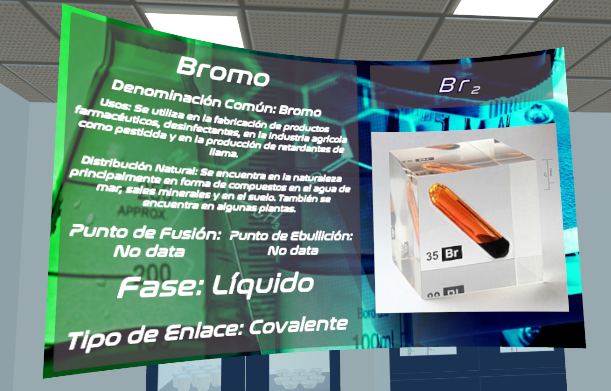
\includegraphics[width=0.6\textwidth, height = 6cm]{img/chapter04/UI_Compuestos.png}
    \caption{IU Compuestos}
    \label{fig:Compuestos_IU}
\end{figure}

\subsection{Área de creación}
Gestiona la combinación de elementos químicos.
\begin{itemize}
    \item \textbf{Indicador de contenido}: Lista dinámica de los elementos colocados en el área de creacón.
    \item \textbf{Validación automática}: Notificación visual que indica si la combinación es válida para generar un compuesto
    \item \textbf{Botón Crear}: Activo únicamente cuando los elementos combinados forman un compuesto válido. Al presionarlo, se genera el compuesto y se actualiza la interfaz.
\end{itemize}
\begin{figure}[thbp]
    \centering
    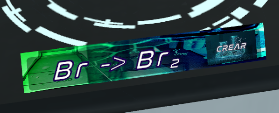
\includegraphics[width=0.6\textwidth, height = 6cm]{img/chapter04/UI_Creacion.png}
    \caption{IU Creación}
    \label{fig:Creación_IU}
\end{figure}
\newpage
\subsection{Teclado numérico interactivo}
Se sincroniza con las ecuaciones químicas mostradas en la IU de información principal, permitiendo la edición en tiempo real.
\begin{figure}[thbp]
    \centering
    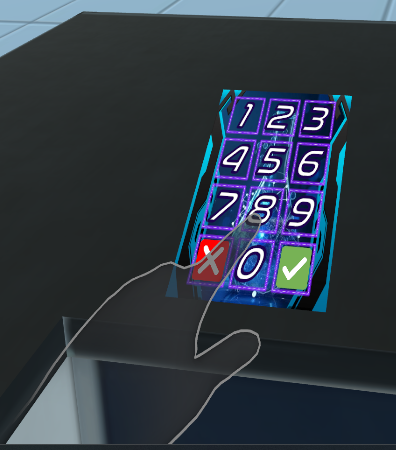
\includegraphics[width=0.4\textwidth, height = 6cm]{img/chapter04/Num_Pad.png}
    \caption{IU Numpad}
    \label{fig:Numpad_IU}
\end{figure}
\subsection{Pantalla final}
Marca la conclusión de un experimento e incluye dos acciones clave:
\begin{itemize}
    \item Repetir experimento: Reinicia el procedimiento desde el principio.
    \item Regresar al hub inicial: Permite al usuario explorar otras opciones o finalizar la sesión.
\end{itemize}
\begin{figure}[thbp]
    \centering
    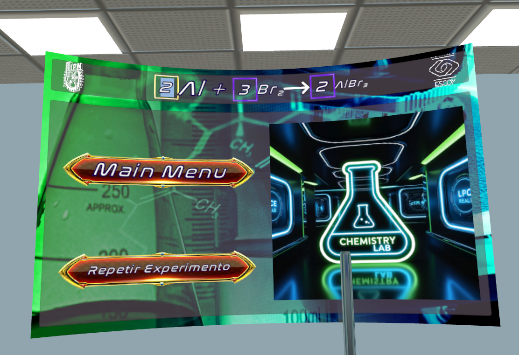
\includegraphics[width=0.6\textwidth, height = 6cm]{img/chapter04/UI_Final.png}
    \caption{IU Pantalla Final}
    \label{fig:Final_IU}
\end{figure}
\newpage
\section{Interacción y Gestos}\label{sec:Gestos}
La interacción dentro del simulador se diseñó para aprovechar las capacidades del seguimiento de manos (hand tracking) ofrecidas por el SDK de Oculus. Esto permite una experiencia intuitiva y natural para el usuario, integrando gestos básicos que emulan acciones físicas reales y simplifican la navegación en el entorno virtual.

\subsection{Interacción con el sistema}
Gracias a las herramientas proporcionadas por el SDK de Oculus, los objetos interactivos fueron configurados con los scripts Grabbable y Hand Grab Interactable. Esto habilita dos formas principales de interacción con los objetos en el entorno:

\begin{itemize}
    \item Sujeción completa: El usuario puede interactuar con los objetos cerrando completamente su mano alrededor de ellos, replicando la acción física de sujetar un objeto.
    \begin{figure}[thbp]
        \centering
        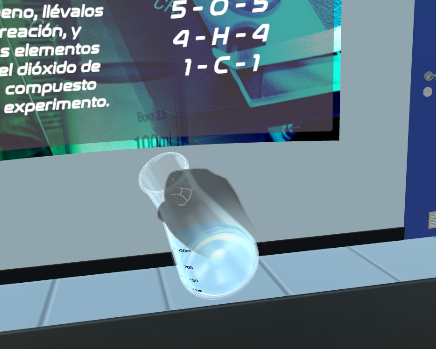
\includegraphics[width=0.6\textwidth, height = 6cm]{img/chapter04/Sujeción_Completa.png}
        \caption{Sujeción completa}
        \label{fig:Sujeción_Completa}
    \end{figure}
    \item Gesto de pinchar: El usuario junta el dedo índice y el pulgar (gesto de pinchar) para manipular objetos más pequeños o realizar interacciones precisas, como seleccionar botones o modificar valores.
    \begin{figure}[thbp]
        \centering
        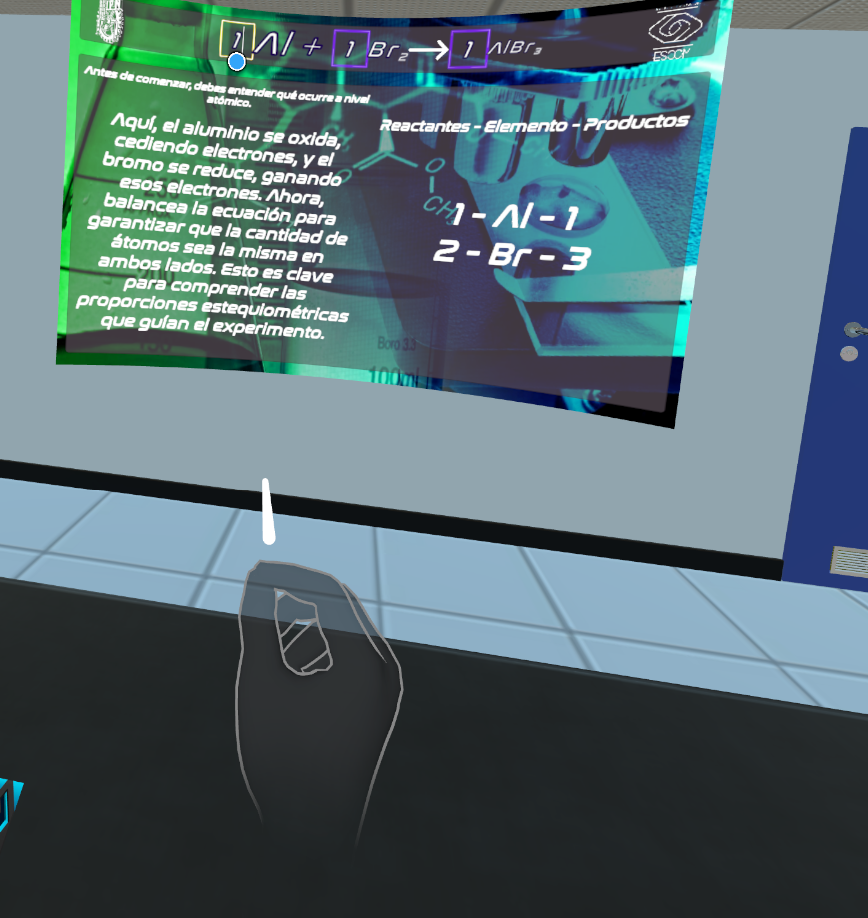
\includegraphics[width=0.6\textwidth, height = 6cm]{img/chapter04/Pinch.png}
        \caption{Gesto de pinchar}
        \label{fig:Pinchar}
    \end{figure}
\end{itemize}

Este gesto específico también se utiliza para interactuar con coeficientes en las ecuaciones químicas y en la selección de botones mediante un apuntador virtual. Esto asegura que las interacciones sean ergonómicas y precisas, incluso en actividades detalladas.

\subsection{Gestos específicos}
Se implementaron gestos adicionales para optimizar la interacción con el laboratorio:
\begin{itemize}
    \item Selección directa con el dedo índice: Al tocar directamente la tabla periódica interactiva o botones cercanos, el sistema reconoce el contacto del dedo índice y activa la acción correspondiente. Esto elimina la necesidad de punteros adicionales para elementos de acceso rápido.
    \begin{figure}[thbp]
        \centering
        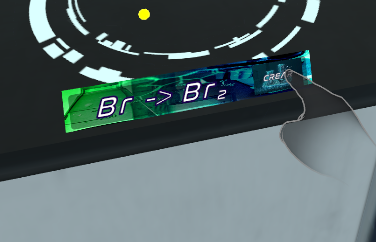
\includegraphics[width=0.6\textwidth, height = 6cm]{img/chapter04/Botones_Cercanos.png}
        \caption{Interacción con botones cercanos}
        \label{fig:Interacción}
    \end{figure}
    \item Centrado del escenario: Se habilitó un gesto general estándar de Oculus para centrar el entorno a la vista del usuario. Este gesto garantiza que el laboratorio virtual se ajuste correctamente al campo de visión, mejorando la comodidad y la orientación espacial del usuario.
    \begin{figure}[thbp]
        \centering
        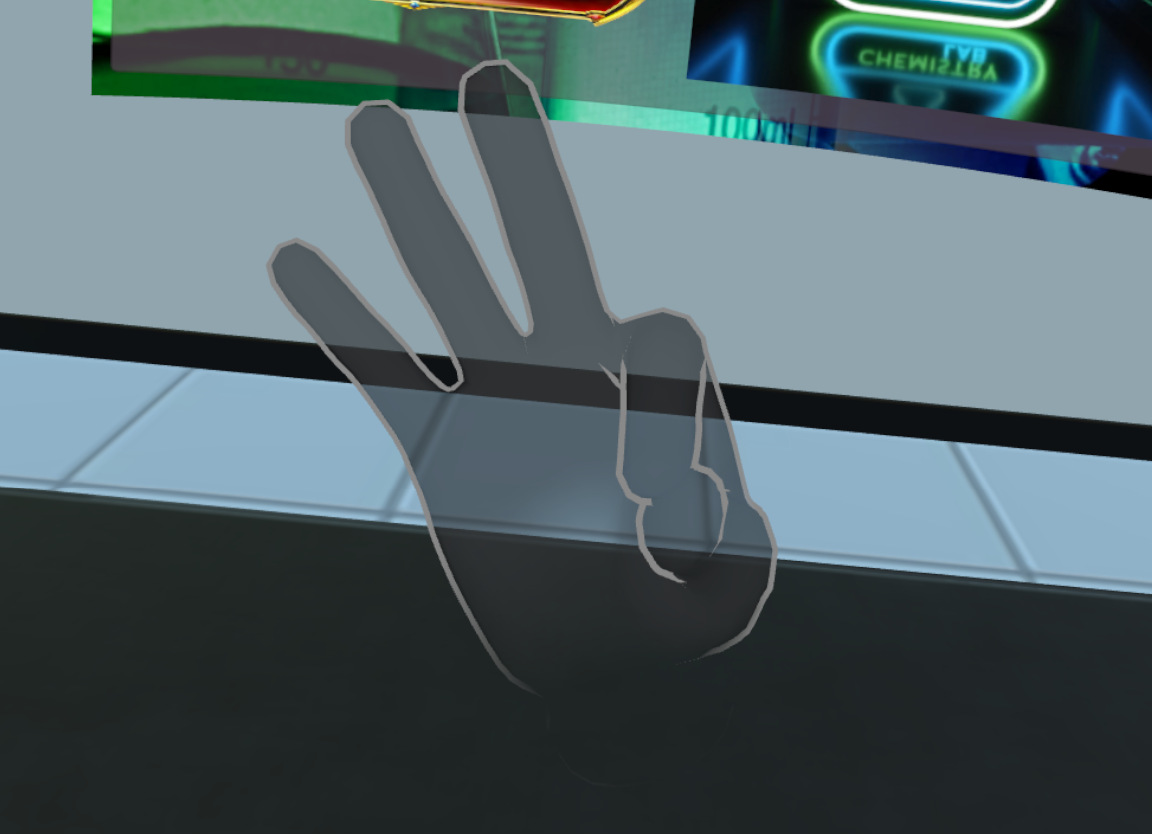
\includegraphics[width=0.6\textwidth, height = 6cm]{img/chapter04/Centrado.png}
        \caption{Gesto para centrar el entorno}
        \label{fig:Centrar}
    \end{figure}
\end{itemize}
El uso de gestos básicos asegura que los usuarios puedan interactuar con el entorno sin requerir controladores físicos. Esto reduce la curva de aprendizaje y mejora la experiencia inmersiva.
\newpage
\section{Integración del SDK de Oculus}
El desarrollo del simulador requirió la implementación del SDK de Oculus, una herramienta clave para habilitar capacidades de realidad virtual inmersiva. Este SDK proporciona un modelo completo que integra cámaras virtuales, controladores y seguimiento de manos (hand tracking) en un entorno preconfigurado.

Para este proyecto, se utilizó el módulo de hand tracking como base principal de interacción, aprovechando su capacidad para detectar y procesar movimientos naturales de las manos sin necesidad de controladores físicos. Este enfoque es particularmente relevante para la interacción con objetos y elementos virtuales descritos en la \autoref{sec:Ambiente_Virtual}: Ambiente Virtual y la \autoref{sec:Gestos}: Interacción y Gestos.

La integración del SDK de Oculus simplificó significativamente el desarrollo del simulador, proporcionando una base sólida para implementar las interacciones y funcionalidades principales sin necesidad de construir estas capacidades desde cero.